% tex image files

\documentclass[leqno]{article}
\pdfoutput=1
\usepackage{graphicx}
\usepackage{color}
\usepackage{amsmath}
\usepackage{amssymb}
\usepackage{tikz}
\usepackage{pgfplots}
\usetikzlibrary{math}
\usetikzlibrary{calc}
\usetikzlibrary{intersections}
\input xy
\xyoption{all}


%this sets up gill (blackboard) letters for reals, complexes, ets.
%  this is appropriate for 10pt (default) document
\font\tengill=msbm10 %scaled 1000
\font\sevengill=msbm7 %scaled 900
\font\fivegill=msbm5 % scaled 700
\newfam\gillfam 
\textfont\gillfam=\tengill
\scriptfont\gillfam=\sevengill
\scriptscriptfont\gillfam=\fivegill
\def\gill{\fam\gillfam}
\def\R{{\gill R}}
\def\C{{\gill C}}
\def\Z{{\gill Z}}
\def\Q{{\gill Q}}

%%%%%%%%%%%%%%%%%%% placement of figures in the margin %%%%%%%%%%%%%%%%%%%%%%%%%
\newcounter{figurecount}
%\renewcommand{\thefigurecount}{\thesection .\arabic{figurecount}}

% command for figures in the margin
% arguments: figure input file name, reference label, figure horizontal
% offset, figure vertical offset, ``Figure'' label horizontal offset,
% ``Figure'' label vertical offset, caption

\newcommand{\marginfig}[7]{
\marginpar{
\refstepcounter{figurecount}      % increment margin figure counter
\label{#2}                        % label the figure
\vspace*{#4}                      % vertical adjustment for figure
\spacer\\
\hspace*{#3}                      % horizontal adjustment for figure
\input{#1}\\
\vspace*{#6}                      % vertical adjustment for ``Figure'' label
\spacer\\
\hspace*{#5}                      % horizontal adjustment for ``Figure'' label
\shortstack{
Figure~\ref{#2}\\ #7
}
\spacer}}
%%%%%%%%%%%%%%%%%%%%%%%%%%%%%%%%%%%%%%%%%%%%%%%%%%%%%%%%%%%%%%%%%%%%%%%%%%%%%%%%

% definitions for algeom text
\newcommand{\Quat}{\mathbb{H}} % <!-- quaternions -->
\newcommand{\Sgroup}{{\rm \bf S}}  % <!-- group of elliptic geometry transformations -->
\DeclareMathOperator{\Rot}{Rot}

%Aut, End, etc. commands
\newcommand{\Aut}{\makebox{Aut}}
\newcommand{\End}{\makebox{End}}
\newcommand{\Hom}{\makebox{Hom}}

% short cut trial
\def\hey{heybaba}

% mapping arrow and isomorphism arrow
\newcommand{\map}{\longrightarrow}
\newcommand{\isomap}{\hspace{1ex}\widetilde{\map}\hspace{1ex}}
\newcommand{\extC}{\hat{\C}}

% ivisible text ``spacer''
\newcommand{\spacer}{\rule[0cm]{0cm}{0cm}}

% load x-y pic
% \input xypic

\newcommand{\ket}[1]{\left| #1 \right\rangle}

\font\biggill=msbm10 scaled  2000
\begin{document}


\begin{center}
{\Large This is for trying out stuff in \LaTeX\ .}
\end{center}


\vspace*{1in}

\medskip

%\input{ngonsymm.pspdftex}
%\input{stereoproj.pspdftex}
%\input{stereoproj2.pspdftex}
%\spacer\hspace*{-1.5in}\input{rotrefl.pspdftex}

\medskip

%%%% commutative diagram for "welldefinedness" proposition
%% \hfill
%% \xymatrix{
%% X \ar[r]^{f} \ar[d]_{\pi} & Y \\
%% X/\!\!\sim \ar@{-->}[ur]_{\overline{f}}
%% }
%% \hfill\spacer

%%%% directed graph example
%% \hfill
%% \xymatrix{
%%   & b & \\
%% a \ar[ur] \ar[dr]  & & c \ar[ul]\ar[ll]\\  
%%   & d \ar[ur] & 
%% }
%% \hfill\spacer

%%%% commutative diagram for conjugate transformation definition
%% \hfill
%% \xymatrix{
%% X \ar[r]^{f} \ar[d]_{\mu} & X \ar[d]^{\mu}\\
%% Y \ar[r]^{g} & Y
%% }
%% \hfill\spacer

%% %%%% commutative diagram for conjugate transformation definition
%% \hfill
%% \xymatrix{
%%   SU(2) \ar[r]^{C_{iH}} \ar[d] & SU(2)\ar[d]\\
%%   \Sgroup \ar[d] & U(\Quat) \ar[d]\\
%% \Rot(S^2) \ar@{<->}[r] & \Rot(S^2_\Quat)
%% }
%% \hfill\spacer

%% %%%% no maps labeled, commutative diagram for integers mod n distributive law
%% \hfill
%% \xymatrix{
%%   \Z_n\times \Z_n \ar[r] \ar[d] & \Z_n\ar[d]\\
%%   \Z_n\times \Z_n \ar[r] & \Z_n 
%% }
%% \hfill\spacer

%% %%%% commutative diagram for integers mod n distributive law
%% \hfill
%% \xymatrix{
%%   \Z_n\times \Z_n \ar[r]^{\text{  add}} \ar[d]_{(\text{times }[x]) \times
%%     (\text{times }[x])} & \Z_n\ar[d]^{\text{times }[x]}\\
%%   \Z_n\times \Z_n \ar[r]_{\text{  add}} & \Z_n 
%% }
%% \hfill\spacer

%%%% lift of complex inversion via stereographic projection
%% \hfill
%% \xymatrix{
%%   S^2 \ar[r]^{R_{X,\pi}} \ar[d]_{s} & S^2 \ar[d]^{s}\\
%%   \extC \ar[r]_{\text{ inversion }} & \extC
%% }
%% \hfill\spacer

%% \hfill
%% \xymatrix{
%%   (a,b,c) \ar[r]^{R_{X,\pi}} \ar[d]_{s} & (a,-b,-c) \ar[d]^{s}\\
%%   \frac{a+bi}{1-c} \ar[r]_{\text{ inversion }} & \frac{a-bi}{1+c}
%% }
%% \hfill\spacer

%% \begin{tikzpicture}
%%   \tikzmath{\t=30;}
%%   \draw[black] (0,0) circle (1);
%%   \draw[red] (\t: {sec(\t)}) circle ({tan(\t)});
%% \end{tikzpicture}

% 2/8/2025 need to control layers
% calculate triangle vertices
% control placement of labels


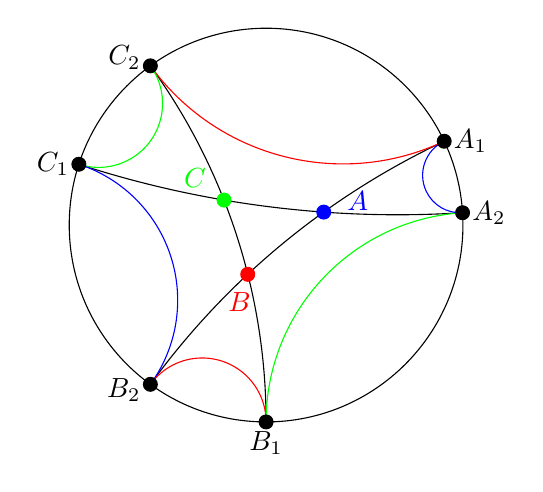
\begin{tikzpicture}[scale=2.5]%[x=2cm,y=2cm]
  \pgfdeclarelayer{fore}
  \pgfsetlayers{main,fore}
  \tikzmath{
    \a1=.07; %     
    \a2=.35; % 
    \b1=.45; % 
    \b2=.65; %     
    \c1=.75; % 
    \c2=0.01; %    
  }
  \tikzmath{
    \A1=\a1*360;
    \A2=\a2*360;
    \B1=\b1*360;
    \B2=\b2*360;
    \C1=\c1*360;
    \C2=\c2*360;    
  }
  \begin{pgfonlayer}{fore}
  %% polar coords is (angle: norm)
  \draw[black] (0,0) circle (1); % boundary circle
  \filldraw[black] (\A1: 1) circle (1pt) node[anchor=west] {$A_1$};
  \filldraw[black] (\A2: 1) circle (1pt) node[anchor=east, yshift=3pt] {$C_2$};
  \filldraw[black] (\B1: 1) circle (1pt) node[anchor=east] {$C_1$};
  \filldraw[black] (\B2: 1) circle (1pt) node[anchor=east, yshift=-2pt] {$B_2$};
  \filldraw[black] (\C1: 1) circle (1pt) node[anchor=north] {$B_1$};
  \filldraw[black] (\C2: 1) circle (1pt) node[anchor=west] {$A_2$};
  \end{pgfonlayer}
  
  % why neg tan?
  
  %%% arc A1 to B2
%  \draw[black] (\A1:1) -- (\B2:1);
  \draw[black, name path=a1b2] (\B2:1) arc ({\B2-90}:{\A1+90}:{(tan((\A1-\B2)/2))}); %
  
  %%% arc A2 to C1
  \draw[black, name path=a2c1] (\C1:1) arc ({\C1-90}:{\A2+90}:{(tan((\A2-\C1)/2))});

  %%% arc B1 to C2
%  \draw[black] (\B1:1) -- (\C2:1);
  \draw[black, name path=b1c2] (\C2:1) arc ({\C2-90}:{\B1+90-360}:{(tan((\B1-\C2)/2))}); %

  \filldraw[blue, name intersections={of=a1b2 and b1c2}]
  (intersection-1) circle (1pt) node[anchor=west, xshift=5pt, yshift=4pt] {$A$};
  \filldraw[red, name intersections={of=a1b2 and a2c1}] (intersection-1)
  circle (1pt) node[anchor=north, xshift=-3pt, yshift=-3pt] {$B$};
  \filldraw[green, name intersections={of=a2c1 and b1c2}]
  (intersection-1) circle (1pt) node[anchor=east, xshift=-3pt, yshift=8pt] {$C$};; 
  
  
  %  \draw[red] ({(\A1+\A2)/2}: {(sec((-\A1+\A2)/2))}) circle  ({(tan((-\A1+\A2)/2))});
  \draw[red] (\A2:1) arc ({\A2-90}:{\A1+90}:{(tan((\A1-\A2)/2))}); % why neg tan?
  
  %  \draw[green] ({(\A2+\B1)/2}: {(sec((-\A2+\B1)/2))}) circle  ({(tan((-\A2+\B1)/2))});
  \draw[green] (\B1:1) arc ({\B1-90}:{\A2+90}:{(tan((\A2-\B1)/2))}); % why neg tan?
  
  %  \draw[blue] ({(\B2+\B1)/2}: {(sec((\B2-\B1)/2))}) circle  ({(tan((\B2-\B1)/2))});
  \draw[blue] (\B2:1) arc ({\B2-90}:{\B1+90}:{(tan((\B1-\B2)/2))}); % 
  
  %  \draw[red] ({(\C1+\B2)/2}: {(sec((\C1-\B2)/2))}) circle  ({(tan((\C1-\B2)/2))});
  \draw[red] (\C1:1) arc ({\C1-90}:{\B2+90}:{(tan((\B2-\C1)/2))}); % 
  
  %  \draw[green] ({(\C2+\C1)/2}: {(sec((\C2-\C1)/2))}) circle  ({(tan((\C2-\C1)/2))});
  \draw[green] (\C2:1) arc ({\C2-90}:{\C1+90-360}:{(tan((\C1-\C2)/2))}); % 
  
  %  \draw[blue] ({(\C2+\A1)/2}: {(sec((-\C2+\A1)/2))}) circle  ({(tan((-\C2+\A1)/2))});  
  \draw[blue] (\A1:1) arc ({\A1-90}:{\C2+90}:{(tan((\C2-\A1)/2))}); %

\end{tikzpicture}




\end{document}












